\clearpage
\section{Step 1: Top-down understanding of a software system}
More often than not, it is the case that software developers have to maintain software projects for which they were not part of the development team. They are expected to understand how the system works and be able to discern any malfunctioning. Maintaining a software that exceeds the size of thousands of lines can prove to be a daunting and complicated task, especially when you are unfamiliar with the source code. It is recommended that an incremental approach is taken when first starting to work on understanding and analysing its source code. \\\\
The majority of software systems have been equipped with source code documentation and useful guides that can help new developers become better acquainted with the system. It is considered a good approach to first take a look at these specific guides and extract as much relevant information as possible, without delving into the source code. The developer can retrieve information about the requirements of the system and its main goals. It is always good to know what are the key drivers of a system because it directly affects implementation details and specifications. This approach is called top-down understanding of a system, because we try to grasp as much relevant information as possible, without delving into the implementation details. \\\\
In this part of the document we present the results of our top-down model for understanding the software system of OptaPlanner. We will tackle some of what we believe are the architecturally significant requirements of the system, have an initial look at the architectural components and establish some initial hypotheses. 
%%%% A S R %%%
\subsection{Defining the ASRs}
\label{subsec:ASR}
Architecturally significant requirements, namely ASR, are those requirements that have a measurable effect on a computer system’s architecture \cite{asrs}. 
They are a subset of the requirements of a system that affect the architecture of a system in measurably identifiable ways. Architecturally significant requirements are used in software design to drive and justify architectural decisions: if not satisfied properly, they contribute to the accumulation of technical debt, which refers to the additional costs that a development team may `suffer' when they decide to (momentarily) choose an easy but short solution, as opposed to a long, but better one.
\paragraph{Quality attributes}
Quality attributes (or non-functional requirements) of a system, can help determine the ASR-s of that system \cite{asrs}.
Given the analysis that we have conducted, mainly based on the user guide for OptaPlanner, we have compiled a list of quality attributes that we deem crucial to the development and maintenance of OptaPlanner.
\begin{itemize}
    \item {\scriptsize\MakeUppercase{Integrability}}\\
    A system that is easy to integrate is one that can be used in collaboration with other (sub-)systems and successfully render the intended functionality.
    OptaPlanner is built on Java$^{\text{TM}}$ and therefore allows for integration with other Java technologies as well \cite{userguide}. According to the user guide, the developers found this quality attribute important, since the OSS was meant to not only be standalone, but also to be integrated with other existing software, and have its functionality easily accessible. Developers who need to solve constraint-solving problems in their systems could use OptaPlanner's algorithms, by integrating them in their own projects.
    
    \item {\scriptsize\MakeUppercase{Adaptability}}\\ 
    % compatibility
    Adaptability is defined as the ability of a system to adjust any necessary aspects so that it can support ongoing changes to the environment. OptaPlanner supports this quality attribute by securing its users compatibility with Standard Java, Enterprise Java and all JVM languages \cite{userguide}.
    
     \item {\scriptsize\MakeUppercase{Backward compatibility}}\\ 
    Backward compatibility is the property of a software system which allows for interoperabilty with an older versions of the system and its operating files. The OptaPlanner team regards backward compatibility 
    
    \item {\scriptsize\MakeUppercase{Configurability}}\\
    Configurability allows for a system to be rearranged and customized according to specific requirements from the user. 
    OptaPlanner supports \verb!xml! filetypes that can be used to determine the optimization algorithm to be used for solving the constraint problem. By changing the solver configuration in the \verb!xml! file, the user can switch to any available optimization algorithm, therefore having the opportunity to customize the system as necessary \cite{userguide}.
    
    \item {\scriptsize\MakeUppercase{Performance}}\\
    Response time refers to the time it would take the system to respond to an input. OptaPlanner uses optimization algorithms in order to supply a good solution in a reasonable time, therefore securing good response times for the user inputs \cite{userguide}.
\end{itemize}
\paragraph{Architecturally Significant Requirements}
\label{par:asrs}
Based on the quality attributes that we were able to define, as well the user guide of OptaPlanner, we can compile a list of the main architecturally significant requirements. 
\begin{enumerate}
    \item \textit{The system should be able to retract relevant information from the} \verb!xml! \textit{files that are created by the users of OptaPlanner.}
    \item \textit{The system should be able to generate at least one solution for the input problem of the end-user.}
    \item \textit{The system should be backward compatible in future releases.}
    \item \textit{The system should give the end-user the opportunity to choose which optimization algorithms should be used to solve the problem in an easy and efficient way.}
    \item \textit{The system should be able to scale, that is, work just as efficiently with large data sets as it works with other data sets}.
\end{enumerate}
\subsection{Architectural Components}
\label{subsec:arch-comp}
Based on our understanding, the user guide document of OptaPlanner is meant to serve as a guide for the end-users of OptaPlanner. That is, it is a document which explains to users step by step how they can define their own problems which OptaPlanner can solve using the optimization algorithms. Therefore, it does not provide an extensive outlook on the implementation details of the system and its architectural components. Since the top-down model is meant to serve as an initial step into the analysis of a software system, we believe that the following steps will guide us into a more extensive view of the internal structures of OptaPlanner. 
Nonetheless, we would like to present a few hypotheses that we discerned from the user guide, which we believe will be relevant for the future analysis. In figure \ref{fig:concept-hypoth} we also depict a conceptual diagram of how we suspect the components to interact together.
\paragraph{Configuration} It appears that configuring \verb!xml! files is very important for the OptaPlanner software. Throughout the entirety of the document, great emphasis is placed on how the user can define the problems he would like to solve with OptaPlanner. We assume that there will be one architectural component whose main concern will with regard to the configuration details.
\paragraph{Optimization algorithms and heuristics} OptaPlanner uses optimization algorithms in order to find optimal solutions for NP-defined problems. From the user guide, we note three main algorithms, namely, Partitioned Search, Exhaustive Search and Local Search. We assume that there is going to be at least one architectural component that is concerned with how the algorithms are defined and how they will be applied to a specific problem. Moreover, some of these algorithms can make use of heuristics, which means that there may be an additional architectural component that is concerned with their definition or perhaps a sub-component of the optimization algorithms.
\paragraph{Score} Another relevant concept that we could discern from the user guide of OptaPlanner is the \textit{score}. This is because the score is used to determine how `optimal' a rendered solution is. We assume that there are architectural components concerned with how the score is defined. 
\paragraph{Constraints} We believe that there is at least one architectural component of OptaPlanner that is concerned with the definition of constraints, how to retract them from a given problem and how to make sure that they are satisfied accordingly. This is because constraints are an intrinsic part of defining an NP-problem and it is also one of the key reasons why OptaPlanner has been developed: to tackle constraint-defined problems.
% \subsection{Hypotheses}
% \begin{enumerate}
%     \item The architectural components of OptaPlanner are clearly defined in the implementation of the system.
%     \item 
% \end{enumerate}
\begin{figure}[H]
    \centering
    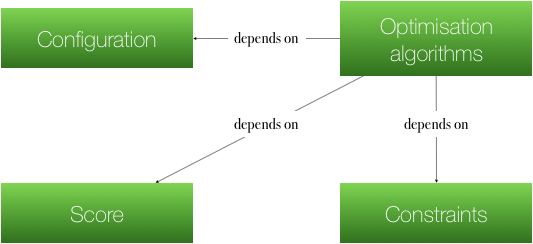
\includegraphics[width=0.4\textwidth]{figures/step2/hypoth.png}
    \caption{A conceptual architectural diagram of the components that we assume will be of importance to the architecture of OptaPlanner.}
    \label{fig:concept-hypoth}
\end{figure}
